\section{Appendix}


\subsection{Risk Matrix}
\label{app:riskmatrix}

\begin{table}[H]
\centering
\caption{Likelihood-Severity-Risk scoring methodology}
\label{tab:likelihood-severity-risk}
\begin{tabular}{@{}cccccc@{}}
\toprule
Severity & \multicolumn{5}{c}{Likelihood}                                                                                                                                    \\ \cmidrule{2-6} 
    & A     & B     & C     & D     & E    \\ \midrule
5   & \yMe  & \yMe  & \rHi  & \rHi  & \rHi \\ 
4   & \yMe  & \yMe  & \rHi  & \rHi  & \rHi \\ 
3   & \yMe  & \yMe  & \yMe  & \rHi  & \rHi \\ 
2   & \gLo  & \gLo  & \yMe  & \yMe  & \rHi \\ 
1   & \gLo  & \gLo  & \gLo  & \gLo  & \yMe \\ \bottomrule
\end{tabular}
\end{table}

\begin{table}[H]
\centering
\caption{Severity scoring methodology}
\label{tab:severity-methodology}
\begin{tabularx}{\linewidth}{llXXX}
\toprule
\multicolumn{2}{l}{\textbf{Severity}} & \textbf{To the People}                                     & \textbf{To the Plant}      & \textbf{To the Environment}      \\ \midrule
1          & Minor             & First Aid                                                  & Superficial Damage         & Slight/no effect                 \\
2          & Moderate          & Medical Care                                               & Repair Needed              & Minor effect                     \\
3          & Serious           & Disabling, Fracture, Hospitalisation (\SI{>24}{\hour})     & Loss of a Process Item     & Short-term Localised Damage      \\
4          & Very Serious      & One Fatality                                               & Local Destruction of Plant & Major/long-term Localised Effect \\
5          & Severe            & Several Fatalities                                          & Complete Destruction       & Multiple Environments Affected   \\ \bottomrule
\end{tabularx}
\end{table}

\begin{table}[H]
\centering
\caption{Likelihood scoring methodology}
\label{tab:likelihood-methodology}
\begin{tabular}{@{}llc@{}}
\toprule
\multicolumn{2}{l}{Likelihood} & Probability ($P$) in 1 year              \\ \midrule
A & improbable & $         P_\mathrm{once} < 0.001 $ \\
B & unlikely   & $ 0.001 < P_\mathrm{once} < 0.01  $ \\
C & possible   & $ 0.01  < P_\mathrm{once} < 0.1   $ \\
D & probable   & $ 0.1   < P_\mathrm{once} < 1     $ \\
E & frequent   & $         P_\mathrm{several} = 1  $ \\ \bottomrule
\end{tabular}
\end{table}

\subsection{Waste Treatment Unit PFD}
\label{app:wastePFD}


\begin{landscape}
\begin{figure}[H]%{h}{0.2\linewidth}
% \vspace{-\intextsep}
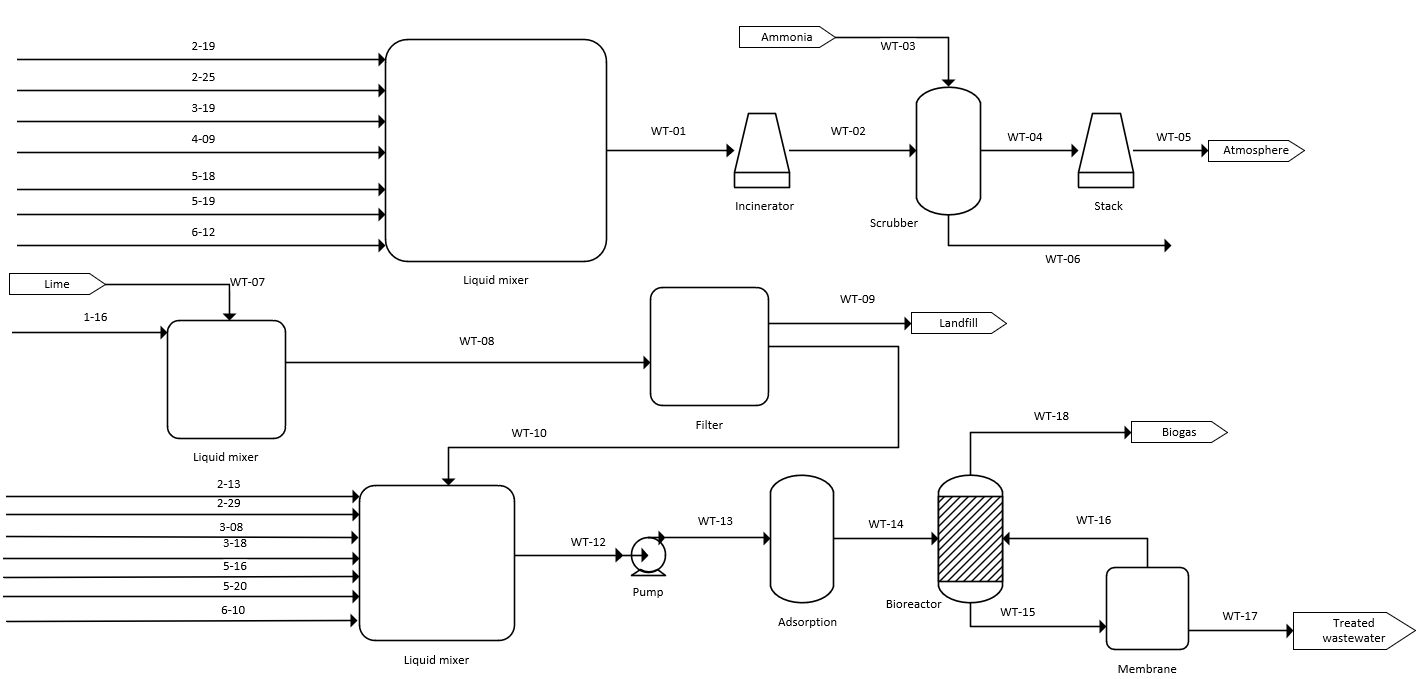
\includegraphics[width=\linewidth]{chapters/5-safety-layout-environment/figures/Waste_PFD.png}
\caption{PFD}
\label{fig:wastePFD}
\end{figure}
\end{landscape}


\subsection{COD Limits}
\label{app:COD}

\begin{table}[H]
\centering
\caption{Liquid waste treatment for BH scenario }
\label{tab:bhwaste}
\resizebox{\textwidth}{!}{%
\begin{tabular}{@{}lllS[table-format=1.2e1,scientific-notation=true,round-mode=figures,round-precision=3]S[table-format=1.2e1,scientific-notation=true,round-mode=figures,round-precision=3]S[table-format=1.2e1,scientific-notation=true,round-mode=figures,round-precision=3]@{}}
\toprule
\multirow[t]{2}{*}{\textbf{Storage}} & \multirow[t]{2}{*}{\textbf{Stream}} & \multirow[t]{2}{*}{\textbf{Component}} & \textbf{Mass Flow} & \multicolumn{2}{l}{\textbf{COD (\si{\mg\per\litre})}} \\ \cmidrule(l){5-6} 
 &  &  & \textbf{(\si{\kg\per\hour})} & \textbf{Before treatment} & \textbf{Post-treatment} \\ \midrule
\multirow[t]{5}{*}{N/A} & \multirow[t]{5}{*}{W1-16} & 3-nitrotoluene & 0.1809 & 14584.8208 & 10.5011 \\
 &  & 2-nitrotoluene & 1.2379 &  &  \\
 &  & 4-nitrotoluene & 1.2748 &  &  \\
 &  & Nitric acid & 46.4544 &  &  \\
 &  & Water & 117.7460 &  &  \\ \midrule
\multirow[t]{15}{*}{1} & \multirow[t]{3}{*}{W3-08} & 3-nitrotoluene & 15.5406 & 151877.9026 & 109.3521 \\
 &  & 2-nitrotoluene & 0.9825 &  &  \\
 &  & 4-nitrotoluene & 11.5268 &  &  \\  \cmidrule(l){2-6}
 & \multirow[t]{3}{*}{W2-13} & 3-nitrotoluene & 2.3176 & 17869.8395 & 12.8663 \\
 &  & 2-nitrotoluene & 0.6452 &  &  \\
 &  & 4-nitrotoluene & 0.3375 &  &  \\  \cmidrule(l){2-6}
 & \multirow[t]{5}{*}{W3-18} & 4-nitrotoluene & 0.6914 & 8946.3289 & 6.4414 \\
 &  & \para-nitrobenzaldehyde & 1.1879 &  &  \\
 &  & Water & 5.3498 &  &  \\
 &  & \para-nitrobenzoic acid & 0.0558 &  &  \\
 &  & 4-Nitrobenzyl alcohol & 0.0013 &  &  \\\cmidrule(l){2-6}
 & \multirow[t]{4}{*}{W5-16} & \para-nitrobenzaldehyde & 1.4411 & 6626.1969 & 4.7709 \\
 &  & \para-nitrobenzoic acid & 0.0002 &  &  \\
 &  & 4-Nitrobenzyl alcohol & 0.1238 &  &  \\
 &  & 4-aminobenzaldehyde & 0.0190 &  &  \\ \midrule
\multirow[t]{9}{*}{2} & \multirow[t]{4}{*}{W5-20} & 4-nitrotoluene & 0.0024 & 19301.6700 & 13.8972 \\
 &  & Water & 3.7635 &  &  \\
 &  & 4-aminobenzaldehyde & 0.1123 &  &  \\
 &  & Formic Acid & 16.1052 &  &  \\ \cmidrule(l){2-6}
 & \multirow[t]{5}{*}{W6-10} & \para-nitrobenzaldehyde & 0.0298 & 7124.4168 & 5.1296 \\
 &  & Water & 17.3148 &  &  \\
 &  & \para-nitrobenzoic acid & 0.7689 &  &  \\
 &  & Formic acid & 3.2008 &  &  \\
 &  & 4-aminobenzoic acid & 0.1163 &  &  \\ \midrule
\multirow[t]{7}{*}{3} & \multirow[t]{7}{*}{W2-29} & 3-nitrotoluene & 0.0280 & 68289.2836 & 49.1683 \\
 &  & 2-nitrotoluene & 0.0154 &  &  \\
 &  & 4-nitrotoluene & 0.0004 &  &  \\
 &  & Nitric acid & 0.0030 &  &  \\
 &  & \ortho-Toluidine & 0.1462 &  &  \\
 &  & Water & 31.3836 &  &  \\
 &  & Methanol & 13.4522 &  &  \\ \bottomrule
\end{tabular}%
}
\end{table}





\begin{table}[H]
\centering
\caption{Liquid waste for BA operation }
\label{tab:wasteBA}
\resizebox{\textwidth}{!}{%
\begin{tabular}{@{}lllS[table-format=1.2e1,scientific-notation=true,round-mode=figures,round-precision=3]S[table-format=1.2e1,scientific-notation=true,round-mode=figures,round-precision=3]S[table-format=1.2e1,scientific-notation=true,round-mode=figures,round-precision=3]@{}}
\toprule
\multirow[t]{2}{*}{\textbf{Storage}} & \multirow[t]{2}{*}{\textbf{Stream}} & \multirow[t]{2}{*}{\textbf{Component}} & \textbf{Mass Flow} & \multicolumn{2}{l}{\textbf{COD (\si{\mg\per\litre})}} \\ \cmidrule(l){5-6} 
 &  &  & \textbf{(\si{\kg\per\hour})} & \textbf{Before treatment} & \textbf{Post-treatment} \\ \midrule
\multirow[t]{5}{*}{N/A} & \multirow[t]{5}{*}{W1-16} & 3-nitrotoluene & 0.1809 & 5442.9619 & 3.9189 \\
 &  & 2-nitrotoluene & 1.2379 &  &  \\
 &  & 4-nitrotoluene & 1.2748 &  &  \\
 &  & Nitric acid & 46.4544 &  &  \\
 &  & Water & 117.7460 &  &  \\ \midrule
\multirow[t]{11}{*}{1} & \multirow[t]{3}{*}{W3-08} & 3-nitrotoluene & 15.5406 & 56679.8626 & 40.8095 \\
 &  & 2-nitrotoluene & 0.9825 &  &  \\
 &  & 4-nitrotoluene & 11.5268 &  &  \\ \cmidrule(l){2-6}
 & \multirow[t]{3}{*}{W2-12} & 3-nitrotoluene & 2.3176 & 6668.9099 & 4.8016 \\
 &  & 2-nitrotoluene & 0.6452 &  &  \\
 &  & 4-nitrotoluene & 0.3375 &  &  \\  \cmidrule(l){2-6}
 & \multirow[t]{5}{*}{W3-18} & 4-nitrotoluene & 0.6914 & 3338.7128 & 2.4039 \\
 &  & \para-nitrobenzaldehyde & 1.1879 &  &  \\
 &  & Water & 5.3498 &  &  \\
 &  & \para-nitrobenzoic acid & 0.0558 &  &  \\
 &  & 4-Nitrobenzyl alcohol & 0.0013 &  &  \\ \midrule
\multirow[t]{4}{*}{2} & \multirow[t]{4}{*}{W6-10} & Water & 435.2568 & 65344.9519 & 47.0484 \\
 &  & \para-nitrobenzoic acid & 19.1210 &  &  \\
 &  & 4-aminobenzoic acid & 2.8916 &  &  \\
 &  & Formic acid & 80.5023 &  &  \\ \midrule
\multirow[t]{7}{*}{3} & \multirow[t]{7}{*}{W2-29} & 3-nitrotoluene & 0.0280 & 25485.1242 & 18.3493 \\
 &  & 2-nitrotoluene & 0.0154 &  &  \\
 &  & 4-nitrotoluene & 0.0004 &  &  \\
 &  & Nitric acid & 0.0030 &  &  \\
 &  & \ortho-Toluidine & 0.1462 &  &  \\
 &  & Water & 31.3836 &  &  \\
 &  & Methanol & 13.4522 &  &  \\ \bottomrule
\end{tabular}%
}
\end{table}


\subsection{Gaussian Plume Model}
\label{app:plumemodel}

\begin{figure*}[H]
    \centering
    \begin{minipage}[t]{0.5\textwidth}
        \centering
        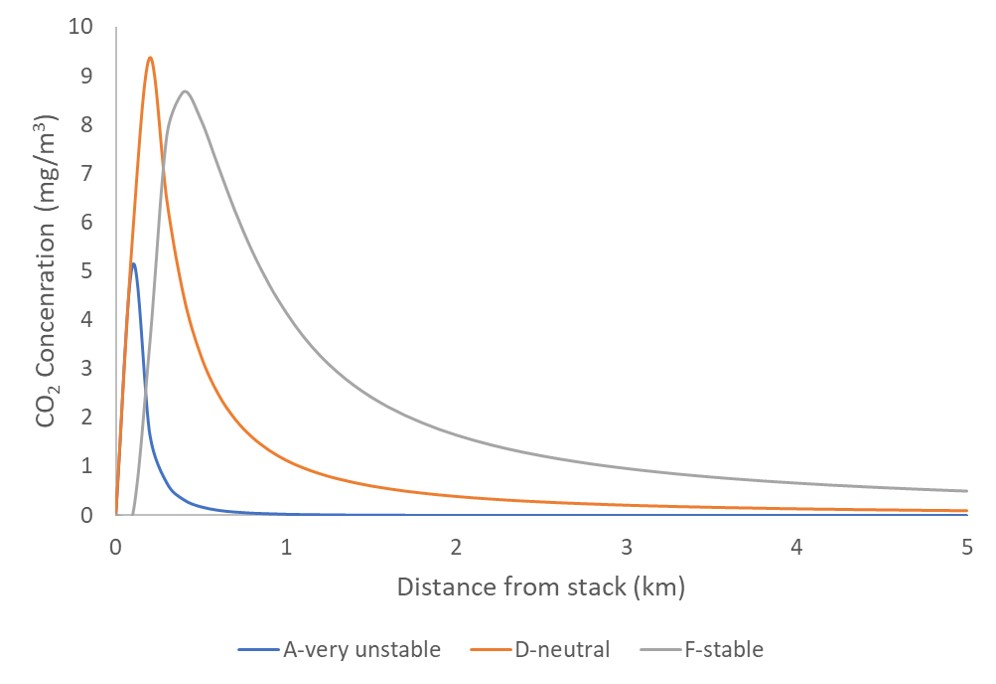
\includegraphics[width=\linewidth]{chapters/5-safety-layout-environment/figures/CO2plumeBA.jpg}
        \caption{\ch{CO2} plume model from BA scenario}
        \label{fig:CO2plumeBA}
    \end{minipage}%
    ~ 
    \begin{minipage}[t]{0.5\textwidth}
        \centering
        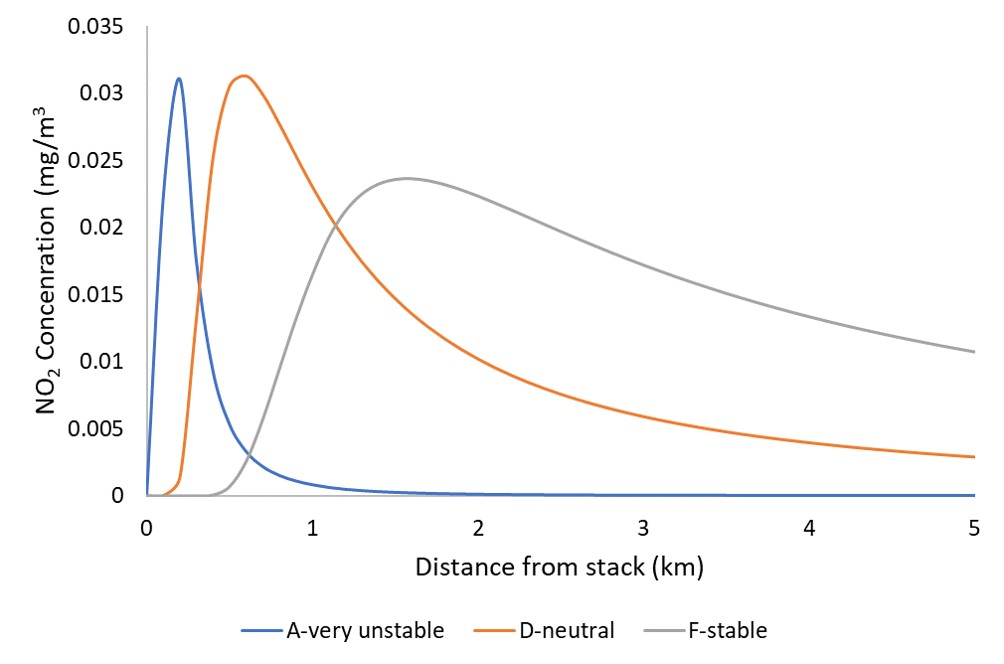
\includegraphics[width=\linewidth]{chapters/5-safety-layout-environment/figures/NO2plumeBA.jpg}
        \caption{\ch{NO2} plume model from BA scenario}
         \label{fig:NO2plumeBA}
    \end{minipage}
    
\end{figure*}


\subsection{Nodes on P\&ID}
\label{app:nodes}

\begin{figure}[H]%{h}{0.2\linewidth}
% \vspace{-\intextsep}
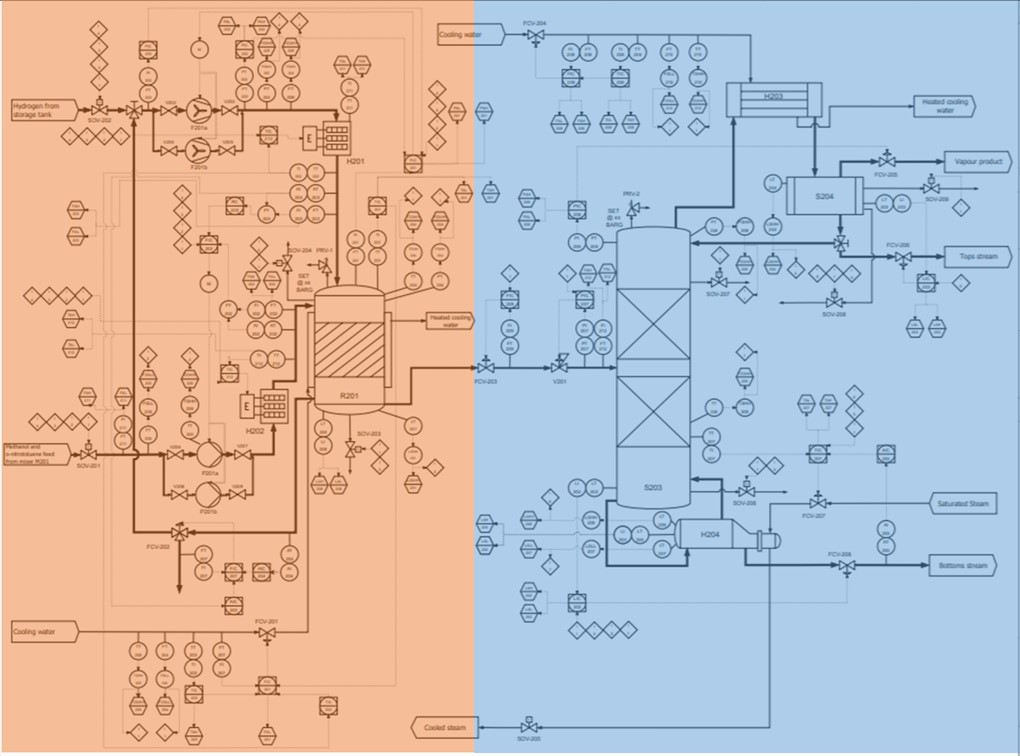
\includegraphics[width=\linewidth]{chapters/5-safety-layout-environment/figures/Node.jpg}
\caption{Nodes of P\&ID: Node 1 (red) and Node 2 (blue)}
\label{fig:node}
\end{figure}


\subsection{Dow's F\&EI}
\label{app:F&EI}

\begin{table}[H]
\centering
\caption{F\&EI and radius of exposure for major process units handling flammable/ unstable materials}
\label{tab:radius}
\begin{tabular}{@{}cS[table-format=3.2]cS[table-format=2.2]@{}}
\toprule\textbf{Process   Unit} & \textbf{F\&EI} & \textbf{Degree of Hazard} & \textbf{Radius of   Exposure (m)} \\\midrule
\multicolumn{4}{c}{Raw   material storage tanks}   
\\\midrule
Toluene                 & 70.88         & Moderate                  & 18.15                             \\
Methanol                & 58.27          & Light                  & 14.92                              \\
Hydrogen gas            & 114.22         & Heavy                     & 29.24                              \\
Formic acid             & 20.00          & Light                     & 5.12                               \\\midrule
\multicolumn{4}{c}{Reactor and separation units}                                                        \\\midrule
R101                    & 88.98          & Moderate                  & 22.78                              \\
S101                    & 35.43          & Light                     & 9.07                               \\
S102                    & 36.80          & Light                     & 9.42                               \\
S103                    & 32.39          & Light                     & 8.29                               \\
S104                    & 82.88          & Moderate                  & 21.22                              \\
S105                    & 36.80          & Light                     & 9.42                               \\
S106                    & 105.18         & Intermediate              & 26.93                              \\
R201                    & 145.22         & Heavy                     & 37.18                              \\
S201                    & 33.85          & Light                     & 8.67                               \\
S202                    & 35.35          & Light                     & 9.05                               \\
S203                    & 33.60          & Light                     & 8.60                               \\
R301                    & 68.92          & Moderate                  & 17.65                              \\
S301                    & 29.40          & Light                     & 7.53                               \\
S302                    & 29.40          & Light                     & 7.53                               \\
S303                    & 29.47          & Light                     & 7.54                               \\
R401                    & 68.92          & Moderate                  & 17.65                              \\
R601                    & 43.17          & Light                     & 11.05                              \\
S601                    & 51.24          & Light                     & 13.12                              \\
S501                    & 29.40          & Light                     & 7.53                               \\
R501                    & 30.83          & Light                     & 7.89                               \\
S502                    & 29.40          & Light                     & 7.53                               \\
S503                    & 49.49          & Light                     & 12.67                              \\
S504                    & 29.40          & Light                     & 7.53                               \\\midrule
\multicolumn{4}{c}{Product   storage tanks}                                                      \\\midrule
o-toluidine             & 19.00          & Light                     & 4.86                               \\\midrule
\multicolumn{4}{c}{Waste   storage tanks}                                                        \\\midrule
W101                    &   70.36           &     Moderate                      &   18.01                                 \\
W102                    &   57.3             &     Light                      &  14.67                              \\\midrule
W103                    &   55.19           &     Light                      &  14.13                              \\\midrule
\multicolumn{4}{c}{Waste process units}                                                        \\\midrule
Neutraliser                    &   46.33            &     Light                      &   11.86                                 \\
Adsorption column                    &   30.50             &     Light                      &  7.81     \\         
Bioreactor                    &   39.65            &     Light                      &   10.15                                 \\
Incinerator                 &   39.55             &     Light                      &  10.13     \\    
Scrubber                 &   39.55             &     Light                      &  10.13     \\\bottomrule

\end{tabular}
\end{table}


